\chapter{Problemi unidimensionali}

\begin{esercizio}[(07/10/2020 n°4)]
   Una particella è vincolata a muoversi all'interno del segmento $0<x<L$ (il potenziale è nullo all'interno del segmento e infinito all'esterno). Calcolare l'energia media sapendo che lo stato della particella è descritto con buona approssimazione dalla funzione d'onda
   \begin{equation*}
      \psi(x)=
      \begin{dcases}
         x & \text{per } 0<x<\frac{L}{2}\\
         L-x & \text{per } \frac{L}{2}<x<L
      \end{dcases}
   \end{equation*}
\end{esercizio}
\begin{soluzione}
   Analizziamo meglio il problema. Il potenziale che agisce sulla particella ha forma
   \begin{equation*}
      V(x)=
      \begin{cases}
         0 & \text{per } x \in [0,L]\\
         +\infty & \text{per } x \notin [0,L]\\
      \end{cases}
   \end{equation*}
   per cui possiamo ignorare cosa succede fuori da $[0,L]$, in quanto la funzione d'onda è ivi identicamente nulla. All'interno di tale segmento invece ha il seguente andamento:
   \begin{figure}[H]
      \centering
      \begin{tikzpicture}
         %assi
         \draw[->] (0,0) -- (0,3) node[above] {$\psi(x)$};
         \draw[->] (0,0) -- (5,0) node[right] {$x$};
         %funzione
         \draw[dashed] (2,2) -- (2,0);
         \draw[thick, blue!60!cyan] (0,0) -- (2,2) -- (4,0);
         \node at (1,-0.5) {I};
         \node at (3,-0.5) {II};
      \end{tikzpicture}
   \end{figure}
   Nella regione I cresce come $x$, mentre nella regione II decresce come $L - x$, in maniera tale che per $x=\frac{L}{2}$ le due funzioni si raccordano.\\
   Il testo ci chiede di calcolare $\expval*{\hat{\mathcal{H}}}$. Ricordiamo che l'hamiltoniana in generale è definita come
   \begin{equation*}
      \hat{\mathcal{H}}=\frac{\hat{p}^2}{2m} + V(\hat{x})
   \end{equation*}
   ma siccome il potenziale all'interno della regione $[0,L]$ è nullo, l'hamiltoniana diventa semplicemente
   \begin{equation*}
      \hat{\mathcal{H}}=\frac{\hat{p}^2}{2m}
   \end{equation*}
   che nella rappresentazione delle coordinate si esprime come
   \begin{equation*}
      \hat{\mathcal{H}}=-\frac{\hbar^2}{2m} \dv[2]{x}
   \end{equation*}
   Sorge tuttavia un problema, in quanto abbiamo una discontinuità nella derivata della funzione: si ha infatti\\
   \begin{minipage}{0.5\textwidth}
      \vspace{0.5cm}
      \begin{equation*}
         \psi'(x)=
         \begin{cases}
            1 & \text{per } x \in \qty[ 0,\frac{L}{2} ]\\[0.2cm]
            -1 & \text{per } x \in \qty[ \frac{L}{2},L ]
         \end{cases}
      \end{equation*}
   \end{minipage}
   \begin{minipage}{0.5\textwidth}
      \begin{figure}[H]
         \centering
         \begin{tikzpicture}
            %assi
            \draw[->] (0,-1.5) -- (0,2) node[above] {$\psi'(x)$};
            \draw[->] (0,0) -- (4.5,0) node[right] {$x$};
            %funzione
            \draw[dashed] (2,1) -- (2,-1);
            \draw[thick, blue!60!cyan] (0,1) node[black,left] {$1$} -- (2,1);
            \draw[thick, blue!60!cyan] (2,-1) -- (4,-1);
            \node[left] at (0,-1) {$-1$};
            \node at (1,-0.5) {I};
            \node at (3,-0.5) {II};
         \end{tikzpicture}
      \end{figure}
   \end{minipage}
   \\[0.4cm]e si evince che c'è una discontinuità in $x=\frac{L}{2}$. Cosa comporta questa discontinuità?
   Quando calcoliamo la derivata prima non ci sono problemi, perché troviamo semplicemente una funzione discontinua, ma quando calcoliamo la derivata seconda la discontinuità nella derivata prima produce qualcosa che dobbiamo sapere come trattare. Il problema sta quindi nel calcolare la derivata seconda in $x=\frac{L}{2}$, che costituisce appunto la discontinuità.\\
   L'idea alla base è quella di adoperare una delta di Dirac. Per fare ciò, poiché la funzione è definita in maniera diversa in regioni diverse, è necessario "incollare" le due funzioni riscrivendo la funzione d'onda come
   \begin{equation*}
      \psi(x)=N \Big\{ x \vartheta\qty( \textstyle \frac{L}{2} \displaystyle - x ) + (L - x) \vartheta\qty( x - \textstyle \frac{L}{2} \displaystyle) \Big\}
   \end{equation*}
   dove $\vartheta$ è la funzione di Heaviside, che è pari a 1 quando il suo argomento è positivo e 0 quando è negativo. In particolare abbiamo
   \begin{gather*}
      \vartheta\qty( \textstyle \frac{L}{2} \displaystyle - x )=
      \begin{cases}
         1 & \text{per } \frac{L}{2} - x > 0 \iff x < \frac{L}{2}\\[0.2cm]
         0 & \text{per } \frac{L}{2} - x < 0 \iff x > \frac{L}{2}
      \end{cases}
      \\[0.2cm]
      \vartheta\qty( x - \textstyle \frac{L}{2} \displaystyle)=
      \begin{cases}
         1 & \text{per } x - \frac{L}{2} > 0 \iff x > \frac{L}{2}\\[0.2cm]
         0 & \text{per } x - \frac{L}{2} < 0 \iff x < \frac{L}{2}
      \end{cases}
   \end{gather*}
   Notiamo che le due funzioni sono praticamente opposte. Il motivo è che così il primo addendo ci definisce la funzione nella regione I (in cui si comporta come $x$) e il secondo nella regione II (in cui si comporta come $L-x$).\\
   Tale scrittura è utile perché sappiamo quanto valgono le derivate delle theta. In particolare, la derivata della theta di Heaviside calcolata in un qualsiasi punto $x_0$ è uguale alla delta di Dirac calcolata nello stesso punto:
   \begin{equation*}
      \dv{x}\vartheta(x-x_0)
      =\delta(x-x_0)
   \end{equation*}
   Ovviamente, se anziché avere $\vartheta(x-x_0)$ abbiamo $\vartheta(x_0-x)$, questa segue le solite regole della derivazione e quindi avremo:
   \begin{equation*}
      \dv{x}\vartheta(x_0-x)
      =\dv{(x_0-x)}{x}\dv{(x_0-x)}\vartheta(x_0-x)
      =\delta(x_0-x)
      =-\delta(x-x_0)
   \end{equation*}
   Calcoliamo ora la $\psi'(x)$: derivando prima la parte regolare (cioè quelle non della theta) e poi l'altra avremo
   \begin{equation*}
      \psi'(x)=N\Big\{ \vartheta\qty( \textstyle \frac{L}{2} \displaystyle - x ) - \vartheta\qty( x - \textstyle \frac{L}{2} \displaystyle) - x\delta\qty( x - \textstyle \frac{L}{2} \displaystyle ) + (L - x)\delta\qty( x - \textstyle \frac{L}{2} \displaystyle ) \Big\}
   \end{equation*}
   dove il segno meno del terzo addendo deriva dalla proprietà enunciata poc'anzi nel caso in cui abbiamo l'argomento della theta invertito.\\
   Sfruttando la proprietà della delta per cui $f(x)\delta(x - x_0)=f(x_0)\delta(x - x_0)$, possiamo riscrivere la parte della derivata in cui figura la delta come\footnote{Attenzione! Quando facciamo questo passaggio dobbiamo comunque tenere la delta, in quanto potremmo poi dover moltiplicare $\psi'(x)$ per un'altra funzione e quella funzione dovrà essere calcolata a sua volta in $\frac{L}{2}$. L'unico modo per eliminare la delta è metterla sotto il segno di integrale.}
   \begin{equation*}
      \textstyle
      - x\delta\qty( x - \frac{L}{2} ) + (L - x)\delta\qty( x - \frac{L}{2} )
      =- \frac{L}{2}\delta\qty( x - \frac{L}{2} ) + \qty(L - \frac{L}{2})\delta\qty( x - \frac{L}{2} )
      =0
   \end{equation*}
   in quanto mettendo in evidenza la delta notiamo che essa è moltiplicata per $0$, e una delta moltiplicata per zero fa zero.\\
   La derivata prima sarà allora
   \begin{equation*}
      \psi'(x)=N\Big\{ \vartheta\qty( \textstyle \frac{L}{2} \displaystyle - x ) - \vartheta\qty( x - \textstyle \frac{L}{2} \displaystyle) \Big\}
   \end{equation*}
   Ribadiamo che tale scrittura significa solo che $\psi'(x)$ vale 1 per $x<\frac{L}{2}$ e $-1$ per $x>\frac{L}{2}$.\\
   Abbiamo quindi scoperto che nella derivata prima non ci sono delta, che era ovvio perché la avevamo già potuta calcolare prima senza problemi. Calcoliamo adesso la derivata seconda:
   \begin{equation*}
      \psi''(x)
      =N \Big\{ \textstyle -\delta\qty( x - \frac{L}{2} ) - \delta\qty( x - \frac{L}{2} ) \Big\}
      =-2N\delta\qty( x - \frac{L}{2} )
   \end{equation*}
   Notiamo che siccome avevamo una discontinuità nella derivata prima allora nella derivata seconda avremo una delta, cosa che non avremmo potuto sapere se avessimo calcolato la derivata di $\psi'(x)$ definendo questa a tratti, in quanto avremmo ignorato la discontinuità, la quale fornisce la delta.\\
   Avendo calcolato la derivata seconda, possiamo calcolare quanto vale $\hat{\mathcal{H}}\ket*{\psi}$: proiettandoci nella base delle posizioni abbiamo
   \begin{equation*}
      \mel*{x}{\hat{\mathcal{H}}}{\psi}
      =-\frac{\hbar^2}{2m}\dv[2]{\psi}{x}
      =-\frac{\hbar^2}{2m} \Bigl[-2N\delta\qty( x - \textstyle \frac{L}{2} ) \Bigr]
      =\frac{\hbar^2N}{m} \delta\qty( x - \textstyle \frac{L}{2} )
   \end{equation*}
   A questo punto non ci resta che calcolare la media $\expval*{\hat{\mathcal{H}}}$: mettendoci di nuovo nella rappresentazione delle coordinate si ha
   \begin{equation*}
      \expval*{\hat{\mathcal{H}}}
      =\mel*{\psi}{\hat{\mathcal{H}}}{\psi}
      =\int_{0}^{L} \dd{x} \psi^*(x) \hat{\mathcal{H}} \psi(x)
      =\frac{\hbar^2 N}{m} \int_{0}^{L} \dd{x} \psi^*(x) \delta\qty( x - \textstyle \frac{L}{2} )
   \end{equation*}
   Notiamo innanzitutto che l'integrale è esteso da $0$ a $L$ anziché da $-\infty$ a $+\infty$ perché al di fuori del segmento la funzione è nulla; inoltre la $\psi(x)$ è definita in un certo modo per $x<\frac{L}{2}$ e in un altro per $x>\frac{L}{2}$, mentre la delta è definita esattamente in mezzo; tuttavia, siccome la funzione è continua nel punto centrale (e non è un caso che lo sia), assumerà lo stesso valore sia da destra che da sinistra, quindi non abbiamo problemi.\\
   Quindi, anziché di dividere la $\psi(x)$ nei due pezzi, sfruttiamo la proprietà della delta per cui quando la mettiamo sotto il segno di integrale con un'altra funzione restituisce la funzione valutata in quel punto e otteniamo
   \begin{equation*}
      \frac{\hbar^2N}{m} \int_{0}^{L} \dd{x} \psi^*(x) \delta\qty( x - \textstyle \frac{L}{2} )
      =\psi^*\qty( \textstyle \frac{L}{2} ) \displaystyle \frac{\hbar^2N}{m}
      =\frac{\hbar^2|N|^2}{m} \frac{L}{2}
   \end{equation*}
   dove nell'ultimo passaggio abbiamo sostituito il valore della funzione per $x=\frac{L}{2}$.\\
   Ci resta solo da calcolare $|N|^2$: imponendo che la funzione sia normalizzata abbiamo
   \begin{equation*}
      1=\int_{0}^{L} \dd{x} |\psi(x)|^2
      =|N|^2 \biggl\{ \int_{0}^{\frac{L}{2}} \dd{x} x^2 + \int_{\frac{L}{2}}^{L} \dd{x} (L - x)^2 \biggr\}
   \end{equation*}
   dove abbiamo spezzato l'integrale in due integrali estesi agli insiemi in cui la funzione è definita in un certo modo. In particolare è possibile ricondurre il secondo integrale al primo operando il cambiamento di variabili $y=L-x$: così facendo avremo $\dd{y}=-\dd{x}$ mentre gli estremi inferiore e superiore di integrazione diventeranno rispettivamente $\frac{L}{2}$ e $0$; se a questo punto invertiamo questi possiamo scrivere
   \begin{equation*}
      1=2|N|^2 \int_{0}^{\frac{L}{2}} \dd{x} x^2
      =2|N|^2 \eval*{\frac{x^3}{3}}_{0}^{\frac{L}{2}}
      =2|N|^2 \frac{L^3}{24}
      =\frac{|N|^2L^3}{12}
      \implies
      |N^2|=\frac{12}{L^3}
   \end{equation*}
   In definitiva
   \begin{equation*}
      \expval*{\hat{\mathcal{H}}}
      =\frac{\hbar^2}{m}\frac{L}{2} \frac{12}{L^3}
      =\frac{6\hbar^2}{mL^2}
   \end{equation*}
   \vspace{0.2cm}\textbf{Ulteriori considerazioni sull'esercizio}\\
   Nel problema appena svolto abbiamo visto che c'era una discontinuità che abbiamo trasformato in una delta. Ma perché è necessaria quella delta? In altre parole, se abbiamo una funzione definita come quella dell'esercizio, avente derivata pari a $1$ per $x \in \qty[0,\frac{L}{2}]$ e $-1$ per $x \in \qty[\frac{L}{2},L]$, perché non possiamo semplicemente scrivere che la derivata seconda è uguale a 0 ma invece dobbiamo usare la delta?\\
   Ricordiamo che abbiamo definito l'energia media come
   \begin{equation*}
      \expval*{\hat{\mathcal{H}}}
      =-\frac{\hbar^2}{2m} \int_{0}^{L} \dd{x} \psi^*(x) \psi''(x)
   \end{equation*}
   e in tale espressione abbiamo due funzioni: una che è ben definita $(\psi)$ e una $(\psi'')$ che diciamo che non è ben definita perché non sappiamo che cosa ci dobbiamo mettere. Possiamo fare una cosa molto semplice: integriamo per parti, ottenendo
   \begin{equation*}
      \int_{0}^{L} \dd{x} \psi^* \psi''
      =\int_{0}^{L} \dd{x} \qty{ \dv{x} \big[ \psi^*\psi' \big] - (\psi')^*\psi' }
      =\big[ \psi^*\psi' \big]_{0}^{L} - \int_{0}^{L} \dd{x} (\psi')^*\psi' 
   \end{equation*}
   Il termine $\big[ \psi^*\psi' \big]$ dà contributo nullo perché $\psi^*$ è pari a 0 sia in $x=0$ che in $x=L$.\\
   Ci resta dunque solo l'integrale in cui abbiamo due funzioni che invece sono ben definite\footnote{Sebbene la derivata prima presenti una discontinuità, ciò non rappresenta un problema in quanto possiamo spezzare l'integrale in due parti: uno che va da $0$ a $\frac{L}{2}$ e uno che va da $\frac{L}{2}$ a $L$, che sappiamo come trattare.}. Non solo: se svolgiamo il calcolo troviamo un risultato diverso da zero, il che significa che l'integrale da cui siamo partiti deve essere diverso da zero anch'esso. Questo è il motivo per cui non possiamo porre semplicemente la $\psi''$ pari a 0, perché troveremmo un risultato in disaccordo a quello ottenuto passando all'integrale.\\
   Tutto questo discorso serve per dire che quando mettiamo qualcosa sotto il segno di integrale dove ci possono essere discorsi di questo tipo (integrazione per parti, ecc.), dobbiamo trattare le funzioni come se fossero delle distribuzioni e quindi fare discorsi ad hoc, come ad esempio in questo caso in cui abbiamo dovuto trattare la derivata di una discontinuità come una delta di Dirac.\\[0.2cm]
   Potevamo anche notare che il valore medio dell'energia in questo caso non può essere nullo. Infatti, se avessimo $\hat{\mathcal{H}}\psi=0$ ciò significherebbe che la derivata seconda della funzione è nulla; se però $\psi''=0$ allora $\psi$ deve essere del tipo $Ax + b$, ma una funzione di questo tipo non può essere nulla agli estremi, in quanto è una funzione strettamente crescente o decrescente. Quindi l'energia non può essere nulla ma per un discorso di condizioni al contorno, perché se proviamo a prendere una funzione avente energia nulla e soddisfacente le condizioni al contorno, l'unica possibilità è $\psi(x)=0$.
\end{soluzione}

\newpage

\begin{esercizio}[(07/10/2020 n°3)]
   Una particella unidimensionale, soggetta al potenziale $V(x)$, si trova nello stato fondamentale di cui è nota la funzione d'onda
   \begin{equation*}
      \psi(x)=Ne^{-\lambda x^4}
   \end{equation*}
   Determinare il potenziale $V(x)$ e l'energia $E_0$ dello stato, misurata rispetto al valore che il potenziale assume nel punto $x=0$. Discutere le principali differenze tra la dinamica classica e quella quantistica in $V(x)$, a parità di energia $E=E_0$.
\end{esercizio}
\begin{soluzione}
   Il problema chiede di determinare il potenziale $V(x)$ e l'energia $E_0$. Siccome però sia il potenziale che l'energia sono definiti a meno di una costante additiva e in questo problema non conosciamo il potenziale quindi non possiamo conoscere tale costante, di fatto il problema chiede di trovare $E_0$ a meno del valore che $V$ assume in $x=0$. Quindi alla fine $E_0$ sarà dara dalla somma di $V(x=0)$ più qualcosa che dobbiamo trovare. La costante additiva sarà fissata in base al valore del potenziale in $x=0$.\\
   Per risolvere il problema sfruttiamo l'informazione che $\psi$ è lo stato fondamentale, quindi in particolare è un autostato dell'hamiltoniana, il che significa che vale
   \begin{equation*}
      \hat{\mathcal{H}}\psi(x)
      =E_0 \psi(x)
   \end{equation*}
   Inoltre conosciamo la forma di $\hat{\mathcal{H}}$, per cui possiamo riscrivere tale equazione nella forma
   \begin{equation*}
      \qty[ \frac{\hat{p}^2}{2m} + V(\hat{x}) ] \psi(x)
      =E_0 \psi(x)
   \end{equation*}
   e a partire da tale relazione possiamo scrivere
   \begin{equation*}
      V(x)\psi(x)=\qty( E_0 - \frac{p^2}{2m} )\psi(x)
   \end{equation*}
   In generale sarà possibile trovare $V(x)$ a patto che $\psi(x)$ sia diversa da zero, e in questo caso la funzione d'onda è diversa da zero per qualsiasi valore di $x$, quindi possiamo scrivere
   \begin{equation*}
      V(x)=\frac{\qty( E_0 - \frac{\hat{p}^2}{2m} )\psi(x)}{\psi(x)}
   \end{equation*}
   Attenzione! Quando scriviamo quest'ultima espressione non possiamo semplificare $\psi(x)$, in quanto $\hat{p}^2$ è un operatore differenziale.\\
   Calcoliamo $-\frac{\hat{p}^2}{2m}\psi(x)$:
   \begin{equation*}
      \begin{split}
         -\frac{\hat{p}^2}{2m}\psi(x)
         =\frac{\hbar^2}{2m} \pdv[2]{\psi(x)}{x}
         & =\frac{\hbar^2}{2m} N \pdv{x} \qty[ -4\lambda x^3 e^{-\lambda x^4} ]
         \\
         & =\frac{\hbar^2}{2m} N \bigl( -12\lambda x^2 + 16\lambda^2 x^6 \bigr) e^{-\lambda x^4}
         \\
         & =\frac{8 \hbar^2 \lambda^2}{m} \qty( x^6 - \frac{3}{4\lambda}x^2 )\psi(x)
      \end{split}
   \end{equation*}
   Notiamo una cosa: siccome il potenziale è proporzionale ad un operatore applicato alla $\psi$ diviso la $\psi$ stessa, la costante di normalizzazione $N$ si semplifica, quindi non è nemmeno necessario il suo calcolo.\\
   Inserendo tale risultato nell'espressione di prima troviamo
   \begin{equation*}
      V(x)=E_0 + \frac{8 \hbar^2 \lambda^2}{m} \qty( x^6 - \frac{3}{4\lambda}x^2 )
   \end{equation*}
   dove abbiamo semplificato la $\psi$ (stavolta lo abbiamo potuto fare perché spuntava fuori a fattore dopo la derivazione).\\
   Se adesso calcoliamo $V(0)$ troviamo che essa è pari a $E_0$. In realtà il discorso è un po' al contrario, perché chiaramente il potenziale non potrà dipendere da $E_0$: scriviamo il potenziale come
   \begin{equation*}
      V(x)=V(0) + \frac{8 \hbar^2 \lambda^2}{m} \qty( x^6 - \frac{3}{4\lambda}x^2 )
   \end{equation*}
   e da ciò deduciamo che $E_0=V(0)$, perché l'esercizio chiedeva specificamente di esprimere l'energia dello stato fondamentale $E_0$ in termini del valore della funzione del potenziale al punto $x=0$.\\
   Questo potenziale avrà un andamento di questo tipo:
   \begin{figure}[H]
      \centering
      \begin{tikzpicture}[scale=1.2]
         \draw[->] (0,-0.5) -- (0,2.2) node[above] {$V(x)$};
         \draw[->] (-2,0) -- (2,0) node[right] {$x$};
         \draw[thick, purple] plot[smooth, domain=-1.2:1.2] (\x, {(\x)^6 - 3/4*(\x)^2});
      \end{tikzpicture}
   \end{figure}
   in quanto per valori grandi di $x$ va come $x^6$, mentre per valori piccoli di $x$ si comporta come $-x^2$. Notiamo che nel grafico abbiamo assunto arbitrariamente $V(0)=0$.\\
   A questo punto facciamo il confronto col caso classico. Calcoliamo la derivata prima e vediamo dove si annulla\footnote{In realtà la funzione avrebbe altri due zeri, che però sono complessi quindi non li consideriamo in quanto in tale problema non hanno senso fisico.}:
   \begin{gather*}
      V'(x)
      =k \qty( 6x^5 - \frac{3}{2\lambda}x )
      =6kx \qty( x^4 - \frac{1}{4\lambda} )
      \\
      \implies
      V'(x)=0 \iff x=0, x=\pm \qty( \frac{1}{4\lambda} )^{\frac{1}{4}} \equiv \pm x_0
   \end{gather*}
   con $k$ un certo coefficiente.\\
   Per $x=0$ abbiamo il massimo, gli altri due valori corrispondono ai due minimi.\\
   Quello che succede ad una particella classica in un potenziale di questo tipo è che quando ha l'energia più bassa sta in un minimo o nell'altro. Infatti, siccome l'energia anche in ambito classico vale $\mathcal{H}=\frac{p^2}{2m} + V$, lo stato di più bassa energia sarà quello avente $p$ e $V$ minimi, che rispettivamente corrispondono ad una particella ferma e che sta ferma in un minimo del potenziale. Quindi le soluzioni di minima energia si hanno per $x=\pm x_0$, dove la particella ha energia pari a $E=V(\pm x_0)$.\\
   Se ciò in meccanica classica ha senso, in meccanica quantistica non può esserci una particella ferma in un minimo del potenziale: il minimo sarà una certa ampiezza.
\end{soluzione}

\newpage

\begin{esercizio}[(08/07/2019 n°2)]
   Una particella unidimensionale è soggetta al potenziale
   \begin{equation*}
      V(x)=-W\delta(x)
   \end{equation*}
   e si trova in uno stato legato.\\
   Dire se è soddisfatto il Teorema del Viriale. Verificare la risposta con un calcolo esplicito dei valori medi di energia cinetica e potenziale.
\end{esercizio}
\begin{soluzione}
   Facciamo una precisazione sulla formulazione del problema: piuttosto che dire che la particella si trova in uno stato legato, sarebbe meglio dire che si trova in un autostato legato. In che senso? Nel senso che se una particella si trova in uno stato legato, questo può essere qualunque: la particella può essere descritta da una funzione d'onda arbitraria fintanto che questa sia normalizzabile, e ciò indipendentemente dall'hamiltoniana. Se poi la funzione d'onda è un'autofunzione allora sarà autostato dell'hamiltoniana, ma se non lo è lo stato va comunque benissimo così com'è. Se ad esempio ci troviamo in un oscillatore armonico e la particella è in uno stato descritto da una gaussiana ma che ha ad esempio la media spostata dal centro o lo scarto quadratico medio più largo di quello che ci si aspetta da un'autofunzione gaussiana, questa non sarà un autostato, ma comunque sarà una funzione d'onda che descrive la particella in maniera ottima.\\
   In poche parole, se il problema dice che la particella si trova in uno stato legato, questo può essere qualunque. Ogni dubbio viene però fugato dalla richiesta successiva, che chiede di dire se è soddisfatto il teorema del Virale: questo infatti in meccanica quantistica è valido solo negli autostati.\\
   In definitiva la prima richiesta del problema è trovare un autostato legato di questa hamiltoniana. Cosa significa legato? Significa che la funzione d'onda è tale che all'infinito vada a zero e quindi si può interpretare come localizzata in una certa regione dello spazio almeno approssimativamente, fatto che garantisce ad essa la qualifica di stato legato.\\
   Attenzione! Stato legato non significa che l'energia è negativa, perché se ad esempio abbiamo una particella di energia $-27$ eV e ridefiniamo l'energia come $E'=E + 30$ eV, la particella adesso avrà energia $E'$ pari a 3 eV, ma se prima si trovava in un stato legato rimarrà comunque in tale stato perché non è cambiata la funzione d'onda, quindi è la stessa particella. Dunque in generale per trovarsi in un stato legato non è necessario che l'energia sia minore di 0, solo che molto spesso noi abbiamo a che fare con potenziali che sono positivi (o che possono essere positivi) come nel caso dell'oscillatore armonico, in cui il potenziale è positivo, l'energia è positiva ma l'oscillatore è evidentemente in un stato legato perché si trova in uno stato localizzato nello spazio (per quanto possa essere localizzata nello spazio una funzione d'onda quantistica, perché chiaramente ha delle code, però comunque la probabilità di trovare la particella è molto maggiore in una certa regione della buca dell'oscillatore armonico).\\
   Studiamo il problema agli autovalori
   \begin{equation*}
      \hat{\mathcal{H}}\ket*{\psi}=E\ket*{\psi}
   \end{equation*}
   dove
   \begin{equation*}
      \hat{\mathcal{H}}=\frac{\hat{p}^2}{2m} + V(\hat{x})
   \end{equation*}
   Facciamo una prima considerazione: sebbene sia vero che quando abbiamo una delta di Dirac non ha senso dire che essa è una funzione che è nulla ovunque e infinita in un punto, è anche vero che è sicuro che se escludiamo dall'intervallo di integrazione la regione in cui la delta è non nulla, nel resto dello spazio è nulla. Ne segue che se abbiamo un problema in cui il potenziale è una delta in $x=0$, escludendo la regione in cui la delta può essere non nulla sotto il segno di integrazione (ossia prendiamo solo le regioni per $x>0$ e per $x<0$), l'equazione agli autovalori si traduce in
   \begin{equation*}
      \frac{\hat{p}^2}{2m}\psi=E\psi
   \end{equation*}
   e quindi la delta rimane nulla in questo senso. Più tecnicamente significa che se anziché considerare l'integrale esteso da $-\infty$ a $+\infty$ lo estendiamo ad un intervallo che non comprende il punto in cui la delta è definita, allora quell'integrale sarà nullo.
   
   In definitiva per $x>0$ e per $x<0$ possiamo risolvere questa equazione, che possiamo riscrivere come
   \begin{equation*}
      \psi''(x)=-\frac{2mE}{\hbar^2}\psi(x)=k^2\psi
      \qqtext{dove}
      k=\sqrt{-\frac{2mE}{\hbar^2}}
   \end{equation*}
   In particolare se $E$ è positivo $k$ sarà immaginario, mentre se $E$ è negativo $k$ sarà reale.
   
   La soluzione più generale di tale equazione è
   \begin{equation*}
      \psi(x)=Ae^{kx} + Be^{-kx}
   \end{equation*}
   Attenzione! Ancora non abbiamo stabilito che è un generico autostato, perché non abbiamo utilizzato il fatto che c'è una delta di Dirac per $x=0$.
   
   Ricordiamo che noi vogliamo cercare stati legati, i quali, proprio per il concetto di stato legato, non possono avere una corrente di probabilità diversa da zero all'infinito. Se infatti lo stato ha una corrente di probabilità che va verso $\pm \infty$, ciò significa che tale stato ha a tutti gli effetti la probabilità che sta andando verso l'infinito e quindi non può essere un stato legato.
   
   Quindi per cercare stati legati potremmo ad esempio calcolare la corrente di probabilità associata a questo stato e imporre che essa sia nulla agli estremi. Quello che troveremmo, come ci possiamo aspettare, è che la funzione d'onda deve essere reale\footnote{Se la funzione d'onda è reale, non c'è nessuna corrente di probabilità.}. Essere una funzione d'onda reale nel nostro caso significa che per $x>0$ e per $x<0$ la funzione deve andare a zero, in quanto si deve annullare la probabilità di trovare la particella. Per annullarsi $k$ deve essere reale, perché se $k$ fosse immaginario rimarrebbe un'oscillazione per $\pm\infty$ che darebbe appunto una corrente. In sostanza agli estremi ci aspettiamo un comportamento del genere:

   \begin{figure}[H]
      \centering
      \begin{tikzpicture}
         \draw[->] (-4,0) -- (4.2,0);
         \draw[->] (0,-0.5) -- (0,2);
         \draw[thick, purple] plot[domain=-4:-1,smooth] (\x,{3*exp(\x)});
         \draw[thick, purple] plot[domain=1:4,smooth] (\x,{3*exp(-\x)});
      \end{tikzpicture}
   \end{figure}

   In definitiva di tutte queste possibili soluzioni, l'unica che rientra del concetto di stato legato è
   \begin{equation*}
      \psi(x)=
      \begin{cases}
         A_{+}e^{-kx} & \text{per } x>0\\
         A_{-}e^{kx} & \text{per } x<0\\
      \end{cases}
   \end{equation*}
   dove $k$ è un numero reale e positivo. Notiamo che con tale definizione la funzione d'onda si annulla per $\pm \infty$.
   
   Potevamo giungere a tale conclusione anche attraverso la seguente considerazione: noi sappiamo che l'energia $E$ è reale, quindi $\sqrt{-E}$ potrà essere soltanto reale o immaginaria. Ne segue che la soluzione generale dell'equazione di Schrödinger del problema in esame (per $x>0$ e per $x<0$) sarà costituita da una somma o di esponenziali reali o di esponenziali oscillanti. Quest'ultime hanno correnti non nulle all'infinito e ivi non si annullano, quindi quelle non possono essere stati legati e dunque necessariamente $k$ deve essere reale e l'energia dovrà essere negativa.
   
   Arrivati a questo punto dobbiamo fare due cose: la prima è determinare $A$ e ciò è semplice perché la funzione deve essere continua; in particolare dovrà esserlo per $x=0$, da cui otteniamo che $A_{+}=A_{-}$.
   
   \E\ da notare che se nel potenziale fosse stata presente la derivata della delta di Dirac, cioè $\delta'(x)$, la funzione d'onda non sarebbe stata continua. Più in generale possiamo dire che
   \begin{itemize}
      \item Se il potenziale non ha singolarità del tipo delta di Dirac o sue derivate, deve essere continua la funzione e la sua derivata prima;
      \item Se nel potenziale c'è una delta di Dirac la derivata prima non deve essere necessariamente continua, ma deve essere comunque continua la funzione d'onda;
      \item Se nel potenziale ci sono derivate prime della delta di Dirac, allora si può perdere pure il requisito di continuità.
   \end{itemize}
   Tornando al problema, abbiamo visto che la funzione è continua, dunque il coefficiente deve essere lo stesso a destra e a sinistra; in altre parole, possiamo scrivere $\psi(x)$ come
   \begin{equation*}
      \psi(x)=Ne^{-k|x|}
      \qqtext{dove}
      k=\sqrt{\frac{2m|E|}{\hbar^2}}, E<0
   \end{equation*}
   con $N$ coefficiente di normalizzazione.
   
   Vediamo adesso che cosa comporta la presenza della delta di Dirac. Vogliamo imporre che l'equazione di Schrödinger sia soddisfatta pure in $x=0$, per cui dobbiamo calcolare la derivata seconda di $\psi(x)$. Vedremo in particolare che non possiamo prendere un valore di $E$ qualsiasi, ma essa sarà legata a $W$.
   
   Innanzitutto riscriviamo la funzione d'onda come
   \begin{equation*}
      \psi(x)=N\qty[ e^{-kx}\vartheta(x) +
      e^{kx}\vartheta(-x) ]
   \end{equation*}
   La derivata prima allora sarà
   \begin{gather*}
      \psi'(x)
      =N\qty[ -ke^{-kx}\vartheta(x) +
      ke^{kx}\vartheta(-x) + e^{-kx}\delta(x) - e^{kx}\delta(x) ]=
      \\
      =N\qty[ -ke^{-kx}\vartheta(x) + ke^{kx}\vartheta(-x) + \delta(x) - \delta(x) ]
      =N\qty[ -ke^{-kx}\vartheta(x) + ke^{kx}\vartheta(-x) ]
   \end{gather*}
   dove nel secondo passaggio abbiamo usato le proprietà della delta per cui $f(x)\delta(x)=f(0)\delta(x)$ e $\delta(-x)=-\delta(x)$.
   
   Facciamo un inciso: in questo caso abbiamo ottenuto due termini contenenti la delta uguali e opposti che quindi si semplificano, ma se avessimo avuto due termini di questo tipo tali da non annullarsi, cioè tali che la loro differenza fosse pari a $\lambda\delta(x)$, nel momento in cui avessimo considerato la derivata seconda avremmo trovato un termine $\lambda\delta'(x)$. La derivata seconda (ce lo dice l'equazione di Schrödinger) è proporzionale al potenziale, pertanto se $\psi'(x)$ ha una delta di Dirac allora $\psi''(x)$ ha una derivata della delta di Dirac che dovrà essere nel potenziale, perché sicuramente questa non potrà essere dovuta a $\hat{p}^2$, il quale è un operatore differenziale e ci dà semplicemente la derivata seconda.\\
   \E\ in questo senso che se abbiamo un potenziale che va come $\delta'(x)$ allora possiamo avere una discontinuità nella funzione stessa, perché se abbiamo una $\delta'(x)$ nel potenziale allora $\psi''(x)$ avrà una $\delta'(x)$, quindi $\psi'(x)$ avrà una $\delta(x)$ e quindi integrando ancora una volta ci sarà un gradino nella $\psi(x)$, il che significa che c'è una discontinuità nella funzione. Quindi in questo senso se abbiamo una $\delta'(x)$ allora possiamo avere una discontinuità nella funzione, perché se non abbiamo una discontinuità nella funzione non spunterà mai una $\delta'(x)$.\\
   Calcoliamo la derivata seconda:
   \begin{gather*}
      \psi''(x)
      =N\qty[ k^2e^{-kx}\vartheta(x) +
      k^2e^{kx}\vartheta(-x) - ke^{-kx}\delta(x) - ke^{kx}\delta(x) ]=
      \\
      =N\big[ k^2e^{-kx}\vartheta(x) + k^2e^{kx}\vartheta(-x) - k\delta(x) - k\delta(x) \big]=
      \\
      =k^2 \underbrace{N\big[ e^{-kx}\vartheta(x) + e^{kx}\vartheta(-x) \big] }_{\psi(x)}- N \big[ k\delta(x) + k\delta(x) \big]
      =k^2\psi - 2Nk\delta(x)
   \end{gather*}
   Avendo usato le stesse proprietà adoperate nel calcolo precedente. Notiamo che questa volta i termini con la delta non si sommano a zero, e ciò proprio perché c'è una discontinuità nella derivata prima.\\
   Se adesso esplicitiamo $k^2$ l'equazione diventa
   \begin{equation*}
      \psi''(x)=N\qty[ -\frac{2mE}{\hbar^2}\psi - 2Nk\delta(x) ]
   \end{equation*}
   Moltiplicando ambo i membri per $-\frac{\hbar^2}{2m}$ otteniamo
   \begin{equation*}
      -\frac{\hbar^2}{2m}\dv[2]{x}\psi=E\psi + \frac{\hbar^2 N k}{m}\delta(x)
   \end{equation*}
   Il termine $-\hbar^2\dv[2]{x}\psi$ è proprio $\hat{p}^2\psi$, per cui portando il termine con la $\delta(x)$ a destra abbiamo
   \begin{equation*}
      \frac{\hat{p}^2}{2m}\psi(x) - \frac{\hbar^2 k N}{m}\delta(x)
      =E\psi(x)
   \end{equation*}
   A questo punto, visto che il nostro obiettivo è confrontare tale espressione con l'equazione di Schrödinger e dunque è necessario un termine che dipenda da $\psi(x)$, facciamo la seguente considerazione: nel termine con la delta abbiamo un fattore $N$, il quale è uguale a $\psi(0)$; poiché in tale termine è presenta una delta, possiamo usare la proprietà adoperata prima ma al contrario e dire che
   \begin{equation*}
      N\delta(x)=\psi(0)\delta(x)=\psi(x)\delta(x)
   \end{equation*}
   In definitiva l'espressione può essere scritta come
   \begin{equation*}
      \qty[ \frac{\hat{p}^2}{2m} - \frac{\hbar^2 k}{m}\delta(x) ]\psi(x)
      =E\psi(x)
   \end{equation*}
   Attenzione! La delta che figura non l'abbiamo calcolata dal potenziale, bensì dalla funzione d'onda: non siamo stati noi a imporre che avessimo un potenziale a forma di delta, abbiamo risolto l'equazione per $x>0$ e per $x<0$, abbiamo imposto che la funzione avesse una certa forma visto che volevamo avere degli stati legatati e infine abbiamo imposto le condizioni di continuità, ma la delta di per sé l'abbiamo trovata dalla derivata della funzione d'onda.\\
   Tale espressione ci dà un'informazione in più sul problema, perché se la confrontiamo con l'equazione di Schrödinger otteniamo
   \begin{equation*}
      - \frac{\hbar^2 k}{m}\delta(x)=-W\delta(x)
      \implies
      W=\frac{\hbar^2 k}{m}
      =\sqrt{\frac{2m|E|}{\hbar^2}} \frac{\hbar^2}{m}
   \end{equation*}
   da cui segue che possiamo avere soltanto un valore dell'energia tale per cui questa uguaglianza sia verificata, il quale si ricava essere
   \begin{equation*}
      W^2=\frac{2m|E|}{m} \hbar^2
      \implies
      |E|=\frac{m W^2}{2\hbar^2}
   \end{equation*}
   Quindi non possiamo avere un'energia arbitraria: essa sarà legata a $W$ tramite questa relazione. In particolare essa sarà l'autovalore dello stato legato.\\
   Passiamo alla seconda parte del problema. Dobbiamo innanzitutto dire se è in generale soddisfatto il teorema del Viriale e poi verificare se è soddisfatto con un calcolo esplicito. Ricordiamo che il teorema del Viriale ci dice che se abbiamo un potenziale del tipo $V=V(\alpha \vb*{r})$ che gode della seguente proprietà
   \begin{equation*}
      V(\alpha \vb*{r})=\alpha^k V(\vb*{r})
   \end{equation*}
   ovvero che è omogeneo di grado $k$ nelle coordinate, allora vale la seguente relazione
   \begin{equation*}
      k\expval*{\hat{V}}=2\expval*{\hat{T}}
   \end{equation*}
   dove $k$ è il grado di omogeneità del potenziale.\\
   Attenzione! La media di $\hat{V}$ e la media di $\hat{T}$ sono rigorosamente calcolate in autostati dell'hamiltoniana, quindi tale relazione non vale in stati che non sono autostati di $\hat{\mathcal{H}}$.\\
   La domanda che adesso ci poniamo è se in tale problema abbiamo un potenziale omogeneo. La risposta è sì: la delta di Dirac gode infatti della proprietà
   \begin{equation*}
      \delta(\alpha x)=\frac{1}{|\alpha|}\delta(x)
   \end{equation*}
   che si può dimostrare nella seguente maniera: consideriamo l'integrale da $-\infty$ a $+\infty$ tra una generica funzione $f$ e $\delta(\alpha x)$ con $\alpha>0$, avremo
   \begin{equation*}
      \int_{-\infty}^{+\infty} f(x)\delta(\alpha x)
      =\int_{-\infty}^{+\infty} \frac{\dd{(\alpha x)}}{\alpha} f\qty( \frac{\alpha x}{\alpha} )\delta(\alpha x)
      =\int_{-\infty}^{+\infty} \frac{\dd{y}}{\alpha} f\qty( \frac{y}{\alpha} ) \delta(y)
      =\frac{f(0)}{\alpha}
   \end{equation*}
   dove abbiamo posto $y=\alpha x$.\\
   Siccome tale relazione vale qualunque sia $f$, allora $\delta(\alpha x)$ deve essere uguale a $\delta(x)/\alpha$.\\
   Quindi in realtà la delta di Dirac in un certo senso è una funzione (sebbene non sia una funzione bensì distribuzione) omogenea di grado $-1$. In conseguenza a ciò, nel nostro caso ci aspettiamo che
   \begin{equation*}
      \expval*{\hat{V}}=-2\expval*{\hat{T}}
   \end{equation*}
   Per verificare tale relazione con un calcolo esplicito operiamo nella seguente maniera: siccome vale la relazione $\expval*{\hat{T}}=E - \expval*{\hat{V}}$, possiamo sostituire nell'equazione di sopra e ottenere
   \begin{equation*}
      \expval*{\hat{V}}=-2\bigl( E - \expval*{\hat{V}} \bigr)
      \implies
      \expval*{\hat{V}}=2E
   \end{equation*}
   Dimostrare che vale tale uguaglianza sarà allora equivalente a dimostrare che vale il teorema del Viriale per il problema in esame. Abbiamo già calcolato $E$, dunque ci resta da calcolare soltanto $\expval*{\hat{V}}$:
   \begin{equation*}
      \expval*{\hat{V}}
      =\int_{-\infty}^{+\infty} \dd{x} -W\delta(x) |\psi(x)|^2
      =-W |\psi(0)|^2
      =-W |N|^2
   \end{equation*}
   e quindi la relazione diventa
   \begin{equation*}
      -W |N|^2=-\frac{m W^2}{\hbar^2}
      \implies
      |N|^2=-\frac{m W}{\hbar^2}
   \end{equation*}
   avendo esplicitato $E$.\\
   A questo punto dobbiamo calcolare la costante di normalizzazione. Ricordando che $\psi(x)=Ne^{-k|x|}$ avremo
   \begin{equation*}
      1
      =|N|^2 \int_{-\infty}^{+\infty} \dd{x} e^{-2k|x|}
      =2|N|^2 \int_{0}^{+\infty} \dd{x} e^{-2kx}
      =\frac{2|N|^2}{2k}
      =\frac{|N|^2}{k}
      \implies
      |N|^2=k
   \end{equation*}
   In definitiva troviamo
   \begin{equation*}
      k=-\frac{m W}{\hbar^2}
   \end{equation*}
   relazione che è in accordo con quanto trovato prima. Dunque il teorema del Viriale è effettivamente valido.
\end{soluzione}

\begin{esercizio}[(14/11/2024 n°1)]
   In una dimensione, un fascio di particelle di massa $m$ proviene da $x=-\infty$, con una intensità di $N$ particelle al secondo, e incide sul grado di potenziale
   \begin{equation*}
      V(x)=
      \begin{cases}
         0 & \text{per } x<0\\
         V & \text{per } x>0\\
      \end{cases}
   \end{equation*}
   con $V>0$. Sapendo che l'energia delle particelle incidenti è $E=V/2$, determinare il numero di particelle che mediamente si trovano nella regione $x>0$ in condizioni stazionarie.
\end{esercizio}
\begin{soluzione}
   Notiamo innanzitutto che il testo ci dice che $N$ è il numero di particelle al secondo, quindi esso non è altro che la corrente $J$. Passiamo adesso ad analizzare la situazione: lo spazio è diviso in una regione I, per $x<0$, in cui il potenziale è nullo e in una regione II, per $x>0$, in cui il potenziale è uguale ad una costante $V>0$. Inoltre il fascio ha energia $E=V/2$:
   \begin{figure}[H]
      \centering
      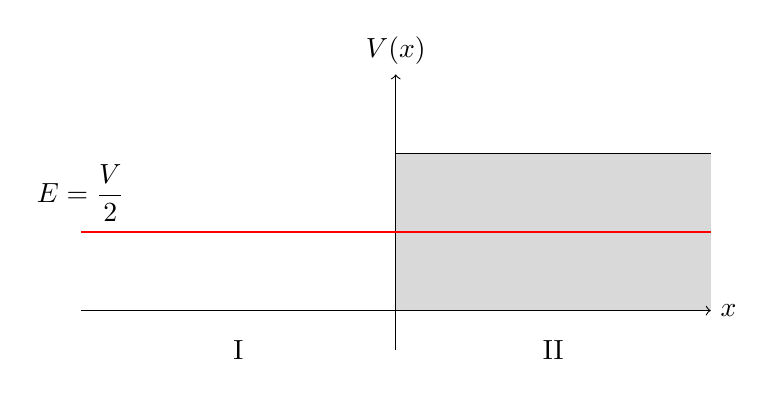
\begin{tikzpicture}
         \filldraw[gray!30!] (0,0) -- (0,2) -- (4,2) -- (4,0) -- cycle;
         \draw[->] (-4,0) -- (4,0) node[right] {$x$};
         \draw[->] (0,-0.5) -- (0,3) node[above] {$V(x)$};
         \draw (0,2) -- (4,2);
         \draw[thick,red] (-4,1) node[left,above,black] {$\displaystyle E=\frac{V}{2}$} -- (4,1);
         \node at (-2,-0.5) {I};
         \node at (2,-0.5) {II};
      \end{tikzpicture}
   \end{figure}
   Poiché nella regione II è presente un potenziale e l'energia è minore di questo, la funzione d'onda assume forma
   \begin{equation*}
      \psi_{\text{II}}(x)=Ce^{-qx}
   \end{equation*}
   dove $C$ è un coefficiente e $Q$ è una costante reale data da
   \begin{equation*}
      q
      =\sqrt{\frac{2m(V-E)}{\hbar^2}}
      =\sqrt{\frac{mV}{\hbar^2}}
   \end{equation*}
   Invece, nella regione I abbiamo un'onda incidente e un'onda riflessa, quindi la funzione d'onda è del tipo
   \begin{equation*}
      \psi_{\text{I}}(x)=Ae^{ikx} + Be^{-ikx}
   \end{equation*}
   dove
   \begin{equation*}
      k
      =\sqrt{\frac{2m(E-V)}{\hbar^2}}
      =\sqrt{\frac{2mE}{\hbar^2}}
      =\sqrt{\frac{mV}{\hbar^2}}
      \equiv q
   \end{equation*}
   in quanto in tale regione $V(x)=0$.
   Riassumendo, la funzione d'onda è data da
   \begin{equation*}
      \psi(x)=
      \begin{cases}
         A e^{iqx} + Be^{-iqx} & \text{per } x<0\\
         Ce^{-qx} & \text{per } x>0
      \end{cases}
      \qq{dove}
      q
      =\sqrt{\frac{mV}{\hbar^2}}
   \end{equation*}
   Facciamo adesso una considerazione sulle correnti. Nella regione I abbiamo una corrente incidente $J_I$ e una corrente riflessa $J_R$, date rispettivamente da\footnote{Precisiamo che con $\psi_I$ intendiamo la funzione d'onda incidente e con $\psi_R$ quella riflessa.}
   \begin{gather*}
      J_I=-\frac{i\hbar}{2m} \qty( \psi_I^*\dv{\psi_I}{x} - \psi_I\dv{\psi_I^*}{x} )
      \qq{dove}
      \psi_I(x)=Ae^{iqx}
      \\
      J_R=-\frac{i\hbar}{2m} \qty( \psi_R^*\dv{\psi_R}{x} - \psi_R\dv{\psi_R^*}{x} )
      \qq{dove}
      \psi_R(x)=Be^{-iqx}
   \end{gather*}
   da cui segue che
   \begin{equation*}
      J_I=\frac{\hbar q}{m}|A|^2
      \qq{,}
      J_R=\frac{\hbar q}{m}|B|^2
   \end{equation*}
   Notiamo adesso che la corrente incidente non è altro che la corrente pari a $N$ fornita dal testo, per cui possiamo uguagliarle e ricavare $|A|^2$, che sarà dunque pari a
   \begin{equation*}
      |A|^2=\frac{mN}{\hbar k}
   \end{equation*}
   Per quanto riguarda la regione II abbiamo una corrente trasmessa $J_T$ che data da
   \begin{equation*}
      J_T=-\frac{i\hbar}{2m} \qty( \psi_T^*\dv{\psi_T}{x} - \psi_T\dv{\psi_T^*}{x} )
   \end{equation*}
   ma siccome $\psi_T=Ce^{-qx}$ è una funzione reale segue che $J_T=0$, da cui a sua volta segue che il coefficiente di trasmissione $T=J_T/J_I=0$. Bisogna però stare attenti al fatto che $T=0$ non implica che non ci siano particelle nella regione II, in quanto potremmo trovarci nella situazione in cui ci sono particelle ma sono ferme, per cui abbiamo corrente nulla.
   
   Detto ciò, imponiamo la continuità della funzione e della derivata in $x=0$. Imponendo la continuità della funzione otteniamo la relazione
   \begin{equation*}
      \left.
      \begin{aligned}
         \psi_{\text{I}}(0)=A+B\\
         \psi_{\text{II}}(0)=C\\
    \end{aligned}
    \right\}
    \implies
    A+B=C
  \end{equation*}
  Imponendo invece la continuità della derivata otteniamo la relazione
   \begin{equation*}
      \left.
      \begin{aligned}
         \psi_{\text{I}}'(0)=iq(A-B)\\
         \psi_{\text{II}}'(0)=-qC\\
      \end{aligned}
      \right\}
    \implies
    i(A-B)=-C
  \end{equation*}
  Mettendo insieme le due relazioni troviamo $B$ in funzione di $A$:
  \begin{equation*}
      i(A - B)=-(A + B)
      \implies
      (i + 1)A=(i - 1)B
      \implies
      B=\frac{i + 1}{i - 1}=iA
  \end{equation*}
  Possiamo ora esprimere $C$ in funzione di $A$:
  \begin{equation*}
   C=A+B=(1+i)A
  \end{equation*}
   A questo punto calcoliamo il numero di particelle nella regione per $x>0$. Scegliendo la normalizzazione tale che il modulo quadro della funzione d'onda corrisponda alla densità, cioè $\rho=|\psi|^2$, tale numero sarà dato da
   \begin{equation*}
      \text{n° particelle}
      =\int_{0}^{+\infty} \dd{x} |\psi|^2
      =|C|^2 \int_{0}^{+\infty} \dd{x} e^{-2qx}
   \end{equation*}
   Poiché
   \begin{equation*}
      |C|^2
      =|1+i|^2|A|^2
      =2|A|^2
      =\frac{2mN}{\hbar q}
   \end{equation*}
   avremo
   \begin{equation*}
      \text{n° particelle}
      =\frac{2mN}{\hbar q} \int_{0}^{+\infty} \dd{x} e^{-2qx}
      =\frac{2mN}{\hbar q} \frac{1}{2q}
      =\frac{mN}{\hbar} \frac{1}{q^2}
      =\frac{mN}{\hbar} \frac{\hbar}{mV}
      =\frac{N\hbar}{V}
   \end{equation*}
   Verifichiamo quanto trovato mediante un'analisi dimensionale. $\hbar/V$ ha le dimensioni di un tempo mentre $N$ è il numero di particelle al secondo, per cui il risultato ottenuto è corretto.
\end{soluzione}